% !TEX encoding = UTF-8 Unicode
% !TEX TS-program = pdflatex
% !BIB program = biber

% toptesti document class
\documentclass[    
    a4paper,
    corpo=12pt, % dimension of basic font
    twoside, % two side optimizes for two-face printing, having chapters open on the right (aka odd numbers), if you don't want blank pages put oneside here
    stile=standard,
    %evenboxes, % not needed, to put supervisors and candidate at the same level
    tipotesi=magistrale,
    numerazioneromana, % roman numbering for appendixes and preambles, up to Table of Contents
    openright, % to force opening on the right for double-sided printing
    cucitura=7mm, % for printing, 7mm should be enough
]{toptesi}



%%%%% 1. GESTIONE LINGUA, CARATTERI E CODIFICA
\usepackage[T1]{fontenc}
\usepackage[utf8]{inputenc}
\usepackage[english, italian]{babel}    % Gestisce entrambe le lingue, l'ultima è quella attiva di default
\usepackage{lmodern}                    % Carica i font stabili suggeriti dal template
\usepackage{hyphenat}                   % Gestione della sillabazione all'interno del testo (usare \nohypenation{parola} per evitare che venga spezzata)
\usepackage{csquotes}                   % Gestione del virgolettato all'interno delle citazioni (usare \enquote{testo} per inserire il testo tra virgolette)
\usepackage{mfirstuc}                   % Gestione della prima lettera maiuscola per parole selezionate (usare \makefirstuc{parola})

%%%%% 2. COLORI (Caricato subito con le opzioni del tuo file)
\usepackage[table, xcdraw]{xcolor}
\usepackage{colortbl}
\definecolor{blupolito}{RGB}{0, 46, 95}

%%%%% 3. GEOMETRIA E SPAZIATURA PAGINA
% Per forzare i margini con la dimensione voluta, togliere il simbolo "%" da \usepackage{geometry} e \geometry{...} qui sotto.
\usepackage{geometry}
%\geometry{a4paper, left = 20mm, top = 25mm, bottom = 25mm}
\usepackage{layout}                     % Utile per visualizzare graficamente il layout completo della pagina (usare \layout) --> solo diagnostica
\usepackage{setspace}                   % Gestione dell'interlinea all'interno del documento (usare \onehalfspacing o \setstretch{1.4})
\usepackage{ragged2e}                   % Miglioramento del controllo sull'allineamento del testo
\usepackage[skip=10pt minus 3pt, tocskip=5pt, indent=0pt]{parskip}     % Gestione della spaziatura tra i paragrafi (skip valore di spazio nominale, il minus indica che se serve per far stare il testo in pagina questo può essere ridotto di 3pt, tocskip è lo spazio nella tabella dei contenuti)

%%%%% 4. GRAFICA, IMMAGINI E CODICE
\usepackage{graphicx}                   % Gestione delle immagini in Latex
\usepackage[export]{adjustbox}          % Estensione funzionalità di centramento e ridimensionamento anche ad altra strutture come tabelle e formule
\usepackage{wrapfig}                    % Gestione della posizione fluida con testo dell'immagine (testo tutto intorno)
\usepackage{subfig}                     % Gestione dei grafici posti all'interno di un'unica figura
\usepackage{svg}                        % Gestione delle immagini in formato svg, garantendo una qualità perfetta
\usepackage{listings}                   % Gestione del codice sorgente, con possibilità di evidenziare la sintassi e di formattare il testo
\usepackage{verbatim}                   % Permette di inserire blocchi di test senza che vengano interpretati come codice Latex

%%%%% 5. MATEMATICA E FISICA
\usepackage{amsmath}                    % Pacchetto per la gestione avanzata della matematica in Latex
\usepackage{amsfonts}                   % Pacchetto per la gestione di font matematici aggiuntivi  
\usepackage{amssymb}                    % Pacchetto per la gestione di font matematici aggiuntivi
\usepackage{bm}                         % Pacchetto per la gestione di simboli matematici in grassetto           
\usepackage{mathtools}                  % Pacchetto per la gestione di simboli matematici (introduce ad esempio \xrightarrow{})
\usepackage{nicefrac}                   % Pacchetto per la gestione di frazioni oblique e compatte (usare \nicefrac{num}{den})
\usepackage{siunitx}                    % Pacchetto per la gestione delle unità di misura (usare \qty{20}{\kilogram\per\cubic\meter})

%%%%% 6. STRUTTURA DELLE TABELLE
\usepackage{array}                      % Pacchetto per la gestione avanzata delle tabelle in Latex
\usepackage{tabularx}                   % Pacchetto per la gestione di tabelle con colonne a larghezza fissa e altre a larghezza variabile
\usepackage{multirow}                   % Pacchetto che permette di unire celle verticalmente in una tabella
\usepackage{longtable}                  % Pacchetto per l'ambiente longtable per la creazione di tabelle che si estendono su più pagine
\usepackage{makecell}                   % Pacchetto per la gestione avanzata delle celle di una tabella, con possibilità di andare a capo
\usepackage{booktabs}                   % Pacchetto per la gestione delle linee orizzontali e verticali in una tabella (\toprule, \midrule, \bottomrule)
\usepackage{ltablex}                    % Pacchetto che unisce tabularx e longtable

%%%%% 7. FORMATTAZIONE CAPITOLI, TITOLI E DIDASCALIE
\usepackage{titlesec}                   % Pacchetto per la gestione avanzata dei titoli di capitolo, sezione e sottosezione
\usepackage[labelfont=bf]{caption}      % Pacchetto per la gestione avanzata delle didascalie di figure e tabelle
\titleformat{\chapter}{\normalfont\huge\bfseries\color{blupolito}}{\thechapter}{1em}{}
\titleformat{\section}{\normalfont\Large\bfseries\color{blupolito}}{\thesection}{1em}{}
\titleformat{\subsection}{\normalfont\large\bfseries\color{blupolito}}{\thesubsection}{1em}{}

%%%%% 8. GESTIONE TABELLE (Definizioni personalizzate dell'utente)
\newcolumntype{P}[1]{>{\centering\arraybackslash}m{#1}} 
\renewcommand{\cellalign}{cc} 
\newcolumntype{Q}[1]{>{\columncolor[HTML]{87cefa}\centering\arraybackslash}m{#1}} 
\renewcommand{\arraystretch}{0.5} 

%%%%% 9. ALGORITMI ED ELENCHI
\usepackage{algorithm}                  % Pacchetto per la gestione dell'ambiente algoritmo (introduce automaticamente anche l'indice apposito)
\usepackage{algpseudocode}              % Pacchetto che introduce un ambiente per scrivere pseudocodice in Latex
\usepackage{enumitem}                   % Pacchetto che permette il controllo di personalizzazione degli elenchi puntati e numerati
\usepackage{lipsum}                     % Pacchetto che introduce il comando \lipsum per generare testo fittizio

%%%%% 10. BIBLIOGRAFIA E CITAZIONI
\usepackage[final]{microtype}           % Rende la spaziatura del testo e della bibliografia perfetta
\usepackage[style=numeric, backend=biber, maxbibnames=9, maxcitenames=2, sorting=none, language=italian, autocite=superscript]{biblatex}           
\let\cite\autocite 

% Configurazione dell'ambiente bibliografia (dal tuo file)
\defbibenvironment{bibliography}
  {\list
     {\printfield[labelnumberwidth]{labelnumber}}
     {\setlength{\labelwidth}{\labelnumberwidth}%
      \setlength{\leftmargin}{\labelwidth}%
      \setlength{\labelsep}{\biblabelsep}%
      \addtolength{\leftmargin}{\labelsep}%
      \setlength{\itemsep}{\bibitemsep}%
      \setlength{\parsep}{\bibparsep}}%
      \renewcommand*{\makelabel}[1]{##1\hss}}
  {\endlist}
  {\item}     

%%%%% 11. COLLEGAMENTI IPERTESTUALI (Sempre per ultimo)
\usepackage{hyperref}                   % Pacchetto per la gestione dei collegamenti ipertestuali (link) all'interno del documento
\usepackage{bookmark}                   % Pacchetto per la gestione dei segnalibri (bookmarks) all'interno del documento
\usepackage{textcomp}                   % Pacchetto per l'introduzione di simboli extra (€, ©, ecc.) prima di hyperref
\usepackage{url}                        % Pacchetto per la gestione corretta dei link internet all'interno di testo e bibliografia

%%%%% 12. GLOSSARI E ACRONIMI
\usepackage[%
    toc,                                % Permette l'inserimento del glossario nell'indice 
    abbreviations,                      % Permette l'inserimento degli acronimi nel glossario
    nonumberlist,                       % Permette di non inserire i numeri di pagina delle occorrenze degli acronimi nel glossario
]{glossaries-extra}                     % Pacchetto per la gestione degli acronimi e dei glossari


%\usepackage{xcolor} % to define colors and use standard CSS names add dvipsnames as option, but it clashes with xcolor loaded in toptesi, pay attention that if it goes in conflict with tikz/beamer, simply use \documentclass[usenames,dvipsnames]{beamer}, along with other custom options when defining the document class
             % File contenente tutti i pacchetti usati nel file

% configuration for glossaries
% convert and load converted glossaries in .tex ,format from .bib

\setabbreviationstyle{long-short-desc} % style before loading resources
% this command sets the style to title for long names of acronyms only in the glossary description, leading to capitalized first-letter for all words
% \glssetcategoryattribute{\glsxtrabbrvtype}{glossname}{capitalisewords} % doesn't work
% resources to load if using a bib file with bib2gls
%\GlsXtrLoadResources[%
% src={glossaries}, % name of the file without extension
% selection=all, % select all the entries
%]
% not needed
%\newglossary*{abbreviation}{Acronyms} % to change the name of this glossary for acronyms

%\renewcommand{\glsclearpage}{\paginavuota} % to allow glossaries to clear pages, done manually is better

% setup for hyperref
\hypersetup{%
    pdfpagemode={UseOutlines},
    bookmarksopen,
    pdfstartview={FitH},
    colorlinks,
    linkcolor={black}, % it is suggested to keep them black, since when printing it it costs per page, and if they have color it's twice the price per page
    citecolor={black},
    urlcolor={black}
  }
%

% setup for svg
\svgsetup{%
    inkscapeformat=pdf, 	% to force usage of PDF
    inkscapelatex=false, 	% to disable latex rendering of text, produces errors
}

% setup for siunitx, it does not work in the summary
\sisetup{%
    detect-all, % to use the same font as for writing when using \num
    mode=text, % to allow it to work also in math mode
    group-separator = {,}, % separator for number grouping
    group-minimum-digits = 3, % minimum number of digits a number must have to be grouped in 3-digit groups
}

% listings colours
\definecolor{rulecolor}{rgb}{0,0,0}
\definecolor{commentcolor}{rgb}{0,0.6,0}
\definecolor{linenumbercolor}{rgb}{0.5,0.5,0.5}
\definecolor{keywordcolor}{rgb}{0,0,0.95}
\definecolor{backcolor}{rgb}{1,1,1}%{0.95,0.95,0.92}
\definecolor{stringcolor}{rgb}{0.58,0,0.82}

% setup for lstlisting
\lstset{ %
	backgroundcolor=\color{backcolor},   % choose the background color; you must add \usepackage{color} or \usepackage{xcolor}; should come as last argument
	basicstyle=\footnotesize,        % the size of the fonts that are used for the code
	breakatwhitespace=false,         % sets if automatic breaks should only happen at whitespace
	breaklines=true,                 % sets automatic line breaking
	captionpos=t,                    % sets the caption-position to bottom
	commentstyle=\color{commentcolor},    % comment style
	extendedchars=true,              % lets you use non-ASCII characters; for 8-bits encodings only, does not work with UTF-8
	frame=single,	                   % adds a frame around the code
	keepspaces=true,                 % keeps spaces in text, useful for keeping indentation of code (possibly needs columns=flexible)
	keywordstyle=\color{keywordcolor},       % keyword style
	%language=VHDL,                 % the language of the code
	numbers=left,                    % where to put the line-numbers; possible values are (none, left, right)
	numbersep=5pt,                   % how far the line-numbers are from the code
	numberstyle=\tiny\color{linenumbercolor}, % the style that is used for the line-numbers
	rulecolor=\color{rulecolor},         % if not set, the frame-color may be changed on line-breaks within not-black text (e.g. comments (green here))
	showspaces=false,                % show spaces everywhere adding particular underscores; it overrides 'showstringspaces'
	showstringspaces=false,          % underline spaces within strings only
	showtabs=false,                  % show tabs within strings adding particular underscores
	stepnumber=1,                    % the step between two line-numbers. If it's 1, each line will be numbered
	stringstyle=\color{stringcolor},     % string literal style
	tabsize=4,	                   % sets default tabsize to 2 spaces
	title=\lstname,                   % show the filename of files included with \lstinputlisting; also try caption instead of title
	inputencoding=utf8,
	literate=
	{á}{{\'a}}1 {é}{{\'e}}1 {í}{{\'i}}1 {ó}{{\'o}}1 {ú}{{\'u}}1
	{Á}{{\'A}}1 {É}{{\'E}}1 {Í}{{\'I}}1 {Ó}{{\'O}}1 {Ú}{{\'U}}1
	{à}{{\`a}}1 {è}{{\`e}}1 {ì}{{\`i}}1 {ò}{{\`o}}1 {ù}{{\`u}}1
	{À}{{\`A}}1 {È}{{\'E}}1 {Ì}{{\`I}}1 {Ò}{{\`O}}1 {Ù}{{\`U}}1
	{ä}{{\"a}}1 {ë}{{\"e}}1 {ï}{{\"i}}1 {ö}{{\"o}}1 {ü}{{\"u}}1
	{Ä}{{\"A}}1 {Ë}{{\"E}}1 {Ï}{{\"I}}1 {Ö}{{\"O}}1 {Ü}{{\"U}}1
	{â}{{\^a}}1 {ê}{{\^e}}1 {î}{{\^i}}1 {ô}{{\^o}}1 {û}{{\^u}}1
	{Â}{{\^A}}1 {Ê}{{\^E}}1 {Î}{{\^I}}1 {Ô}{{\^O}}1 {Û}{{\^U}}1
	{œ}{{\oe}}1 {Œ}{{\OE}}1 {æ}{{\ae}}1 {Æ}{{\AE}}1 {ß}{{\ss}}1
	{ű}{{\H{u}}}1 {Ű}{{\H{U}}}1 {ő}{{\H{o}}}1 {Ő}{{\H{O}}}1
	{ç}{{\c c}}1 {Ç}{{\c C}}1 {ø}{{\o}}1 {å}{{\r a}}1 {Å}{{\r A}}1
	{€}{{\euro}}1 {£}{{\pounds}}1 {«}{{\guillemotleft}}1
	{»}{{\guillemotright}}1 {ñ}{{\~n}}1 {Ñ}{{\~N}}1 {¿}{{?`}}1
}


% biblatex setup
% generally 9000 is ok, if higher than 10000 it's bad
% If you want to break on URL numbers
\setcounter{biburlnumpenalty}{9000}
% If you want to break on URL lower case letters
\setcounter{biburllcpenalty}{9000}
% If you want to break on URL UPPER CASE letters
\setcounter{biburlucpenalty}{9000}
       % File contenente alcune istruzioni e comandi personalizzati per i pacchetti


% Percorso per stampare sul main text il logo del Politecnico in maniera semplificata
\newcommand{\thesisuniversitylogo}{images/logo/polito_logo_2021_blu-2-2}

% Permette di rinominare l'indice dei contenuti
\addto\captionsitalian{
  \renewcommand{\contentsname}%
    {Indice}%
}

% Permette di introdurre righe commentate nello pseudocodice (con il simbolo del triangolo) tramite il comando \LineComment{testo}
\algnewcommand{\LineComment}[1]{\State \(\triangleright\) #1}

% Permette di gestire al meglio valore assoluto e norma
\DeclarePairedDelimiter\abs{\lvert}{\rvert}%
\DeclarePairedDelimiter\norm{\lVert}{\rVert}%

% Permette di modificare automaticamente l'altezza delle stanghe di valore assoluto e norma in base al contenuto
\makeatletter
\let\oldabs\abs
\def\abs{\@ifstar{\oldabs}{\oldabs*}}
%
\let\oldnorm\norm
\def\norm{\@ifstar{\oldnorm}{\oldnorm*}}
\makeatother
         % File contenente comandi e istruzioni aggiuntive per ambienti come quelli matematici e algoritmici



\newcommand{\thesistitle}{Titolo della tesi}
\newcommand{\thesissubtitle}{Eventuale sottotitolo} % not strictly necessary, leave empty if not needed
\newcommand{\thesiscandidatename}{Federico}
\newcommand{\thesiscandidatesurname}{Cecchini}
\newcommand{\thesissupervisoronename}{Stefano}
\newcommand{\thesissupervisoronesurname}{Primatesta}
\newcommand{\thesissupervisortwoname}{Lorenzo}
\newcommand{\thesissupervisortwosurname}{Colli}
\newcommand{\thesisdate}{Mese Anno}
\newcommand{\thesiscourse}{Corso di Laurea Magistrale in Ingegneria Aerospaziale}
\newcommand{\academicYear}{A.a. 2026/2027}
\newcommand{\thesisuniversity}{Politecnico di Torino}
\newcommand{\thesiscandidatetext}{Candidati}
\newcommand{\thesissupervisortext}{Relatori}      % File con le informazioni per il frontespizio


% fontsize is {size}{spacing}\family
\newcommand {\institutionfont}{\fontsize {20}{30}\selectfont}
\newcommand {\divisionfont}{\fontsize {12}{20}\rmfamily}
\newcommand {\pretitlefont}{\fontsize {16}{16}\rmfamily}
\newcommand {\customtitlefont}{\fontsize {24}{28}\selectfont}
\newcommand {\customsubtitlefont}{\fontsize {14}{28}\selectfont}
% {iwona}{bx}{n}}
\newcommand {\fixednamesfont}{\fontsize {12}{16}\mdseries}
\newcommand {\namesfont}{\fontsize {12}{16}\mdseries}
\newcommand {\footfont}{\fontsize {15}{18}\rmfamily}
      % File per la gestione del font e delle dimensioni del testo nelle varie sezioni

\addbibresource{bibliography.bib}   % Richiamo del file di bibliografia in formato bibtex

% for glossary entry
% @entry{bird,
%     name={bird},                          % Nome completo e scorciatoia per richiamare il termine nel testo
%     description = {feathered animal},     % Spiegazione per la pagina del glossrio 
%     see={[see also]{duck,goose}}          % Se sono presenti termini correlati all'acronimo
% }

% if this bib file does not work, try using \input{file.tex}
% where all the \newabbreviation commands have been inserted
% containing all the definitions

% Possibili comandi:
% \gls{parola} permette di stampare il termine (la prima volta esteso e con l'abbreviazione tra parentesi, le successive volte solo l'abbreviazione)
% \Gls{parola} permette di stampare il termine con la prima lettera maiuscola (la prima volta esteso e con l'abbreviazione tra parentesi)
% \GLS{parola} permette di stampare il termine tutto in maiuscolo (la prima volta esteso e con l'abbreviazione tra parentesi)
% \glspl{parola} permette di stampare il termine al plurale
% \glsxtrshort{parola} permette di stampare solo l'abbreviazione (anche se è la prima volta che si usa)


% if you want to use also description for the abbreviations/acronyms, you should use bib2gls and define all the entries in a bib file, which is incompatible with Overleaf
\newacronym{DBMS}{DBMS}{Database Management System}              % File per la gestione del glossario e degli acronimi
%\makeglossaries


% Inizio documento
\begin{document}


\overfullrule=0.00001pt % Permette di disegnare un quadrato nero nelle parole che vanno in overfull, utile per capire dove si trova il problema, da togliere alla fine

%\emergencystretch=1em % to allow some stretching in the lines to avoid overfull boxes, also in bibliography, eventually can be used only before bibliography or in the preamble for the whole document, not needed if using biblatex configuration in most cases
               % File che contiene istruzioni utili per il debug

%% TOPTESI DEFAULT FRONTPAGE, IGNORED
%\ateneo{\thesisuniversity} % university name
%\logosede[5cm]{\thesisuniversitylogo} % logo, square brackets contain the height

%\titolo{\thesistitle} % title
%\sottotitolo{Metodo dei satelliti medicei} % subtitle

% place/remove a slash \\ to put the name on the following line or after Master Degree Course
%\corsodilaurea{\thesiscourse} % course name


%~251197 % id number is not needed

%\candidato{\thesiscandidatename~\textsc{\thesiscandidatesurname}} % candidate

% using tabular we can have more than 1 supervisor under the same column
%\relatore{\tabular{@{}l}%
%    \xmakefirstuc{\thesissupervisoronetitle}~\thesissupervisoronename~\textsc{\thesissupervisoronesurname}\\[0.4ex]
%    \xmakefirstuc{\thesissupervisortwotitle}~\thesissupervisortwoname~\textsc{\thesissupervisortwosurname}\\[0.4ex]
%    \xmakefirstuc{\thesissupervisorthreetitle}~\thesissupervisorthreename~\textsc{\thesissupervisorthreesurname}
%    \endtabular}
%\terzorelatore{Name}

% in this way we have Academic Year without stile=classica, so without lines
%\sedutadilaurea{\textsc{Academic~Year} 2019-2020}% per la laurea magistrale
% for PoliTo there is only month year
%\sedutadilaurea{\thesisdate}% per la laurea magistrale
% PhD
%\esamedidottorato{Novembre 1610}
%\ciclodidottorato{XV}

% offset for binding, the smaller the better
%\setbindingcorrection{3mm}


%\iflanguage{english}{%
	%\retrofrontespizio{This work is subject to the Creative Commons Licence}

%	\CorsoDiLaureaIn{\thesislevel's Degree Course in\space}

%	\TesiDiLaurea{\thesislevel's Degree Thesis}

%	\InName{in}
%	\CandidateName{\xmakefirstuc{\thesiscandidatetext}}% or Candidates
%	\AdvisorName{\xmakefirstuc{\thesissupervisortext}}% or Supervisor
	%\TutorName{Tutor}
	%\NomeTutoreAziendale{Internship Tutor}

	%\NomePrimoTomo{First volume}
	%\NomeSecondoTomo{Second Volume}
	%\NomeTerzoTomo{Third Volume}
	%\NomeQuartoTomo{Fourth Volume}
%}{}

\lstdefinelanguage{JavaScript}{
  keywords={break, case, catch, continue, debugger, default, delete, do, else, finally, for, function, if, in, instanceof, new, return, switch, this, throw, try, typeof, var, void, while, with, const, import, async, await},
  morecomment=[l]{//},
  morecomment=[s]{/*}{*/},
  morestring=[b]',
  morestring=[b]",
  sensitive=true
}

\lstset{
   language=JavaScript,
   extendedchars=true,
   basicstyle=\footnotesize\ttfamily,
   showstringspaces=false,
   showspaces=false,
   numbers=left,
   numberstyle=\footnotesize,
   numbersep=9pt,
   tabsize=2,
   breaklines=true,
   showtabs=false,
   captionpos=b
}       % File con la configurazione della toptesi (qui usato solo per definire l'utilizzo di codici JavaScript)


% EDIT THE thesis_info.tex FILE, NOT THIS ONE!
\newgeometry{top=4cm,left=3cm,right=3cm,bottom=4cm,heightrounded}
\begin{titlepage}
\centering
%
\includegraphics[width=110mm]{\thesisuniversitylogo}\\
%
\vspace{\stretch{2}}
%
{\institutionfont \textbf{\thesisuniversity} \par}
%
\vspace{\stretch{1}} % changing this number and the others changes the proportion
%
{\divisionfont \thesiscourse \par}
{\divisionfont \academicYear \par}
\iflanguage{english}{
    {\divisionfont Graduation Session \thesisdate \par}
}{\divisionfont Sessione di laurea \thesisdate \par}
%

\vspace{\stretch{4}}
%
{\customtitlefont \textbf{\thesistitle} \par}
{\customsubtitlefont \textbf{\thesissubtitle} \par}
%
\vspace{\stretch{4}}
%
\makebox[\textwidth]{\null\hfill\def\arraystretch{1.1} % to change the spacing change this number
\begin{minipage}[t]{.4\textwidth}
    \begin{tabular}[t]{@{}ll@{}}
        \fixednamesfont \thesissupervisortext: & \\
         & \namesfont \thesissupervisoronename~\thesissupervisoronesurname \\
         & \namesfont \thesissupervisortwoname~\thesissupervisortwosurname %\\
         % uncomment if you need a third supervisor
         % & \namesfont \thesissupervisorthreename~\thesissupervisorthreesurname
    \end{tabular}
\end{minipage}
%
\hfill
%
\begin{minipage}[t]{.4\textwidth}
\begin{tabular}[t]{@{}ll@{}}
    \fixednamesfont \thesiscandidatetext: & \\
     & \namesfont \thesiscandidatename~\thesiscandidatesurname
\end{tabular}
\end{minipage}\hfill\null}\\
%
\vspace{\stretch{1}}
%
\end{titlepage}

\restoregeometry
        % File che permette di implementare il frontespizio nel pdf

\paginavuota                        % Introduce una pagina vuota necessaria per la stampa fronte-retro

\frontmatter                        % Permette di iniziare la sezione di introduzione --> numerazione apposita in numeri romani

% abstract if needed
% \begin{abstract}
%     % abstract, choose between abstract and summary
% \end{abstract}

% to create blank pages for openright in frontmatter
% use one of the following two methods
% 1) use the following three lines
%\phantom{0} % needed otherwise cleardoublepage does not clean the page because it sees it empty
%\cleardoublepage
%\thispagestyle{empty} % to have empty page, without numbers
% 2) or
\paginavuota % to manually create a blank page

% summary (uncomment until "end summary" if needed)
%\sommario
%% only the text for the summary

Lorem ipsum dolor sit amet, consectetur adipiscing elit, sed do eiusmod tempor incididunt ut labore et dolore magna aliqua. Sed arcu non odio euismod lacinia at quis risus sed. Tempor commodo ullamcorper a lacus vestibulum. Sed elementum tempus egestas sed sed risus. Netus et malesuada fames ac turpis. Sed blandit libero volutpat sed cras ornare arcu dui vivamus. Vel pharetra vel turpis nunc eget lorem dolor. Iaculis nunc sed augue lacus viverra vitae congue. Orci eu lobortis elementum nibh. Faucibus nisl tincidunt eget nullam non nisi est sit. Ante metus dictum at tempor commodo ullamcorper. Tempus quam pellentesque nec nam. Nulla malesuada pellentesque elit eget gravida.


% $400\times$ is nicer than 400x


%\phantom{0}
%\cleardoublepage
%\thispagestyle{empty}
% end summary

\ringraziamenti                     % Comando per introdurre le caratteristiche del template per la pagina dei ringraziamenti
% acknowledgements

Lorem ipsum dolor sit amet, consectetur adipiscing elit, sed do eiusmod tempor incididunt ut labore et dolore magna aliqua. Tristique senectus et netus et malesuada fames ac turpis. Pretium nibh ipsum consequat nisl vel pretium lectus quam. Urna molestie at elementum eu facilisis sed odio morbi quis. Sed egestas egestas fringilla phasellus faucibus scelerisque eleifend. At in tellus integer feugiat. Mauris rhoncus aenean vel elit scelerisque mauris pellentesque pulvinar. Commodo sed egestas egestas fringilla. Nunc lobortis mattis aliquam faucibus purus in massa. Facilisis magna etiam tempor orci eu lobortis elementum nibh. Elementum curabitur vitae nunc sed velit dignissim. Neque volutpat ac tincidunt vitae. Massa id neque aliquam vestibulum morbi blandit cursus risus at. Porta non pulvinar neque laoreet suspendisse interdum consectetur. Turpis in eu mi bibendum. Ut tristique et egestas quis ipsum suspendisse. Integer quis auctor elit sed vulputate mi sit amet. Viverra nam libero justo laoreet sit amet cursus.

\vspace*{5\baselineskip}    % File contenente il testo dei ringraziamenti

\paginavuota

\tableofcontents                    % Indice dei contenuti per i capitoli

\listoftables                       % Indice dei contenuti per le tabelle 

\listoffigures                      % Indice dei contenuti per le figure

% actually abbreviation is the name used for acronym in glossaries-extra
% title sets the name
% type tells the type of glossary to print
% style overrides the global style
% here we are printing only abbreviations
% printunsrtglossary if using record, otherwise printglossary is ok
%\paginavuota
%\printunsrtglossary[style=altlist,title=Glossario,type=\glsxtrabbrvtype]

% Qui si potrebbe inserire anche la lista dei simboli se necessaria e il glossario 



\glsresetall            % Comando per resettare acronimi e glossario 

%\glsunsetall            % Comando per far comparire unicamente sigla abbreviata anche al primo richiamo (usando il semplice \gls{})
  % File con alcune istruzioni per la gestione del passaggio a testo principale (reset indice acronimi usati in introduzione e abstract)

\mainmatter                             % Comando che permette di iniziare la parte di testo principale --> si resetta la numerazione delle pagine e la si imposta in numeri arabi

% Qui andrebbe inserita l'inizio della parte se il file è così suddiviso (occorre inserire una pagina bianca prima del capitolo perché non può essere sul retro di questa)

% Inserire i singoli capitoli della tesi 

\chapter{Introduzione}


\chapter{Machine learning e reti neurali}

% Possibile introduzione al machine learning generico

All'interno del complesso insieme di algoritmi ascrivibili all'ambito del Machine Learning, una delle classi più promettenti al fine di effettuare operazioni di regressione si rivela essere quella delle \emph{reti neurali}. Questi modelli, infatti, data la loro struttura, sono in grado di analizzare enormi quantità di dati non elaborati, identificando autonomamente pattern complessi, spesso fortemente non lineari, ed appredendo da essi. 

L'ispirazione alla base di tali algoritmi proviene dal funzionamento del cervello umano, in grado di analizzare in pochi millisecondi problemi complessi e, sfruttando anche informazioni passate immagazzinate all'interno delle singole sinapsi, generare una risposta ottimale. Naturalmente, replicarne la capacità di ricordare nel tempo grandi quantità di dati e l'elevato numero di interconnessioni, che definiscono con che livello di sofisticatezza si svolgono le operazioni necessarie, è quasi impossibile, data l'enorme potenza di calcolo che sarebbe necessaria. Tuttavia, le reti neurali sono in grado di migliorare con l'esperienza, analogamente al cervello, in una fase definita training e risultano persino più rapide nel processare le informazioni. 

A livello strutturale, quindi, l'elemento elementare risulta essere il \emph{neurone}, in grado di ricevere in input molteplici dati, elaborarli internamente tramite l'utilizzo di una funzione lineare, caratterizzata da specifici pesi e bias, e, in base alla funzione di attivazione prescelta, produrre un output. Solitamente si generano dei cosiddetti \emph{layer di neuroni}, che si interfacciano vicendevolmente. Una rete neurale, per essere definita tale, deve avere almeno due layer fondamentali: l'\emph{input layer}, che riceve direttamente i dati grezzi forniti all'algoritmo, e l'\emph{output layer}, che produce il risultato ricercato. Normalmente, tuttavia, a questi si aggiungono uno o più layer intermedi, definiti \emph{hidden layers}. Essi, infatti, sono necessari per aumentare  la capacità della rete di estrarre relazioni non lineari dai dati, pur aumentando la complessità e la potenza di calcolo associati al modello. Inoltre, in caso siano presenti almeno 3 layer complessivi, non ci si riferisce più all'ambito del semplice machine learning, bensì si entra in quello che viene definito \textbf{deep learning}.   

\begin{figure}[h!]
    \centering
    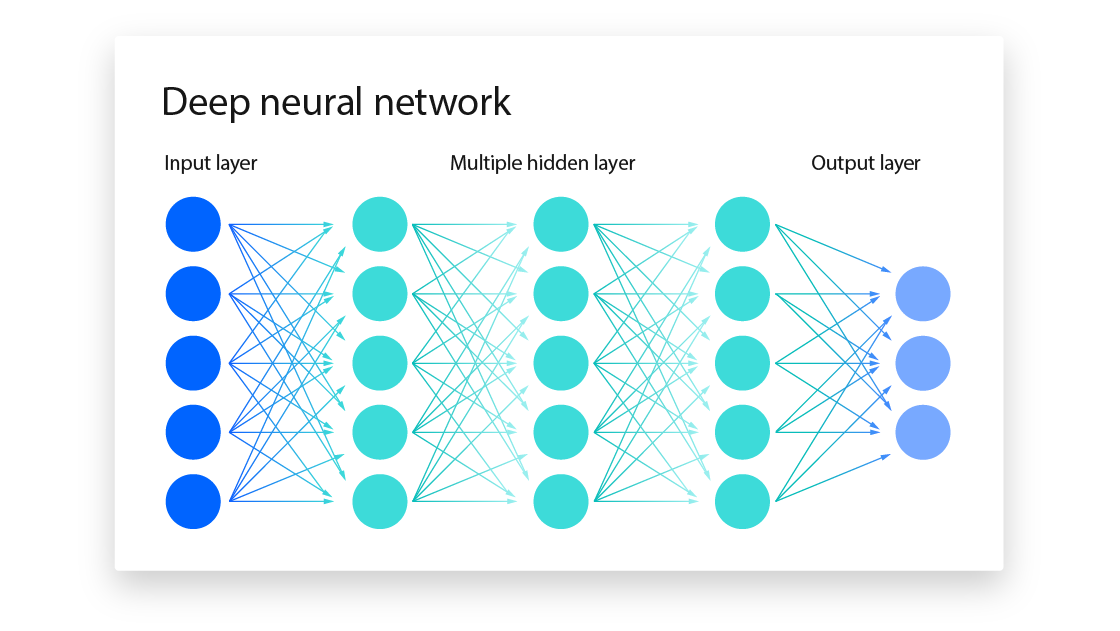
\includegraphics[width=0.8\linewidth]{images/NN/Struttura_base_DL.png}
    \caption{Struttura tipica di un algoritmo di Deep Learning\cite{IBM_NN}}
    \label{fig:DL_struct}
\end{figure}

% Qui si potrebbe aggiungere anche uno schema di funzionamento e spiegazione di forward e back propagation

\section{Elementi rete neurale}

Conclusa questa prima introduzione alle reti neurali, presentata schematicamente in \emph{Figura} \ref{fig:DL_struct}, è necessario analizzarne il funzionamento più nel dettaglio, in modo tale da comprendere, anche a livello matematico, come si arriva all'output desiderato. Nelle sezioni che seguiranno, pertanto, verranno descritti e valutati individualmente tutti gli elementi che compongono una rete neurale. 

\subsection{Neuroni}

Come anticipato, l'entità fondamentale di una rete neurale è il neurone, che risulta estremamente simile a livello concettuale rispetto alla controparte biologica, come si può notare dal confronto mostrato in \emph{Figura} \ref{fig:confronto_neuroni}. Più dettagliatamente, un neurone tradizionale riceve informazioni da altri neuroni tramite i dendriti, le elabora internamente e produce un output sotto forma di impulsi eletttrici, trasmessi ad altri elettroni attraverso le sinapsi poste alla fine della coda. Particolare attenzione va riservata al meccanismo di trasmissione delle informazioni, che avviene grazie a dei messaggeri chimici, chiamati \textit{neurotrasmettitori}, generati a partire dal segnale elettrico prima di giungere alle sinapsi. 

Un neurone artificiale, pur non necessitando della presenza di tutti questi elementi complessi, è in grado di replicare fedelmente il comportamento appena descritto. Ogni neurone, infatti, riceve informazioni da tutti i neuroni del layer che lo precede, le elabora tramite l'utilizzo di una funzione lineare e di una funzione di attivazione e produce un singolo output, trasmesso al layer successivo. Naturalmente, analogamente a ciò che avviene nel cervello umano, non tutti i percorsi tra neuroni impattano allo stesso modo per giungere al miglior output possibile. Ogni connessione, pertanto, presenta uno specifico peso $w_{i}$, determinato durante la fase di apprendimento della rete. 

Un neurone, pertanto, produce un primo output $z$ effettuando una somma pesata degli $n$ valori ricevuti in input:

    \begin{center}
        $z = \sum_{i=1}^{n} w_{i}*x_{i} + b$ \ \ \ $(2.1)$
    \end{center}

All'interno di questa relazione, sviluppata da Rosenblatt per il Perceptron, una delle prime reti neurali, compare un termine aggiuntivo oltre ai pesi, noto come \textit{bias}. Anch'esso viene modificato durante la fase di addestramento della rete al fine di ottimizzare il risultato del modello. 

\begin{figure}[h!]
    \centering
    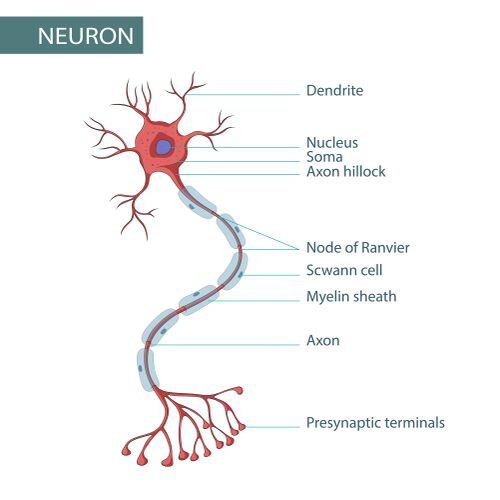
\includegraphics[width=0.5\linewidth]{images/NN/Neurone_bio_2.png}
    \caption{Confronto tra neurone biologico\cite{jpg_neurone_bio} e artificiale}
    \label{fig:confronto_neuroni}
\end{figure}


\subsection{Funzione di attivazione}

L'output prodotto nella prima fase di analisi da parte del neurone, necessita di un ulteriore passaggio prima di essere trasmesso ai layer successivi. Occorre, infatti, normalizzare il valore ottenuto e aggiungere non linearità al modello, potendo così approssimare pattern più complessi.

% Classificazione attivazione

\subsection{Learning Rule}



\section{Algoritmi tipici}

\chapter{Algoritmi di navigazione}

\section{Kalman Filters}

Tradizionalmente, la navigazione di un drone autonomo si basa su approcci model-based, che simulano il comportamento dinamico di quest'ultimo in base alle misurazioni derivanti dai sensori presenti a bordo. 

(dovuti ai sensori, caratterizzati da imperfezioni che nascono al momento della loro costruzione, e al modello del drone, che è soggetto per forza di cose ad approssimazioni rispetto alla controparte reale)

\section{Literature Review}

A seguito del rapido sviluppo avuto dal settore dell'intelligenza artificiale e, in particolare, del machine learning negli ultimi anni, sono comparse in letteratura numerose architetture in grado di unire i vantaggi degli approcci model-based e data-driven. Tra di esse, si distinguono metodologie atte a migliorare i vari aspetti che concorrono alla precisione finale della navigazione, tra cui la calibrazione iniziale dei sensori, l'accuratezza della stima del vettore velocità, input del metodo utilizzato, e la correzione del vettore posizione stimato dal filtro di Kalman. 

% Inserire possibili architetture per categoria: 
                                                % BeamsNet e derivati, UDON, SMNN per miglioramento velocità
                                                % VM-PMC-EKF e tutti quelli per miglioramento diretto navigazione
                                                % Algoritmi solo ML per navigazione

\subsection{Calibrazione e denoising sensori}

Il processo di fusione tra dati inerziali e DVL genera enormi vantaggi in termini di precisione della navigazione in assenza di strumenti di posizionamento esterni come il GNSS. Tuttavia, la riuscita di questo approccio dipende fortemente dal corretto allineamento tra i sistemi di riferimento dei sensori coinvolti. In letteratura sono presenti molti approcci di stampo tradizionale che propongono possibili soluzioni a tale problematica, sebbene mostrino tutti notevoli margini di miglioramento in termini di precisione e velocità di convergenza. Un importante passo in avanti può essere fatto impiegando algoritmi di machine learning, che permettono di trattare grandi volumi di dati caratterizzati da relazioni non-lineari. Damari et al.~\cite{AlignNet} nel suo lavoro presenta un approccio, basato su una rete neurale convoluzionale 1D, in grado di generare una matrice di rotazione tra i due sistemi di riferimento in questione. Nel tentativo di migliorare tale approccio, sempre Damari et al.~\cite{ResAlignNet} presenta un algoritmo differente, questa volta basato su layer convoluzionali raccolti in vari residual blocks. % Da chiedere poi quanto bisogna andare nel dettaglio con le descrizioni

Altri approcci si concentrano su differenti problematiche, riguardanti la struttura intrinseca dei sensori. Yampolsky et al.~\cite{DCNet} propone un approccio data-driven per la calibrazione del DVL, basato su una rete neurale convoluzionale molto complessa. % Si potrebbe cercare anche approcci su denoising che compaiono nel paper di Cohen sulla review


\subsection{Miglioramento precisione navigazione}

Uno dei parametri chiave per la navigazione dell'AUV è senza dubbio il vettore della velocità fornito dal Doppler Velocity Log, che fornisce una misura correttiva per le componenti stimate, tramite integrazione numerica classica, dal filtro di Kalman. Tradizionalmente, il passaggio dalle misurazioni grezze del sensore alle componenti del vettore finale, avviene attraverso l'utilizzo di un \textbf{Least Square Estimator}. % Si potrebbe approfondire di più l'LS concentrandosi sui lati negativi 

Tuttavia, un simile approccio presenta diverse criticità, tra cui l'eccessiva sensibilità alla presenza di outliers nelle misurazioni e la necessità di definire un modello del sensore, producendo ulteriori incertezze nei dati. Una soluzione a tale problematica passa, ovviamente, attraverso l'utilizzo di tecniche di machine learning, basate unicamente sull'addestramento tramite dati misurati sperimentalmente. Una delle architetture più versatili ed efficienti si rivela sicuramente essere il BeamsNet, proposta da Cohen et al.~\cite{BeamsNet} nel 2022. Questo approccio permette di migliorare il livello di precisione della velocità fornita al filtro di Kalman tramite l'integrazione delle misurazioni IMU e DVL. In particolare, questo viene fatto grazie all'utilizzo di un filtro 1DCNN, un dropout layer e diversi FC layers posti in successione. I risultati presentati sono sicuramente incoraggianti, con un miglioramento rispetto all'utilizzo dell'LS estimator del 62.28 \% in termini di Root Mean Squared Error della velocità. Un approccio simile è stato presentato da Zhang et al.~\cite{UDON} nel 2025. All'interno di questa rete neurale l'architettura utilizzata risulta essere molto simile a quella legata al BeamsNet, con la fondamentale aggiunta di un layer LSTM; quest'ultimo, infatti, consente di catturare meglio le dipendenze temporali a lungo termine, ottenendo così un miglioramento più ampio rispetto alla prima rete. I test, seppur basati su dati provenienti da missioni svolte in ambiente lacustre, nettamente meno indicativo rispetto ai test in mare per la valutazione della robustezza della rete, mostrano un miglioramente pari al 69 \% in termini di RMSE sulla velocità stimata rispetto all'LS estimator.

\chapter{Costruzione Dataset}

%%%%% Scaletta %%%%%%%%

% - Descrizione dataset utilizzato e come lo ho costruito: con indicazioni su missioni simulate scelte e motivazioni

% - Excursus sul simulatore utilizzato

% - Descrizione processo di validazione e testing

%%%%%%%%%%%%%%%%%%%%%%%

\section{Preparazione simulatore}

Per una prima valutazione delle correlazioni statistiche e delle prestazioni della rete neurale, come si è visto, è stato utilizzato un dataset prodotto internamente all'azienda e basato su un'unica traiettoria rettilinea, ripetuta in diverse condizioni ambientali e di navigazione. Data la natura stessa del dataset, tuttavia, non risulta possibile dimostrare le effettive prestazioni della rete in traiettorie più articolate, simili a quelle che il drone si troverà ad affrontare in missioni reali. 

Pertanto, si è reso necessario ampliare tale dataset, introducendo nuove traiettorie, pur ripetendo lo stesso pattern di selezione delle possibili configurazioni ambientali e di navigazione. Esso, infatti, risulta già essere un ottimo compromesso tra la necessità di addestrare la rete neurale a gestire il maggior numero di situazioni differenti e il ridurre la potenza di calcolo necessaria all'intero processo. 

Per ogni traiettoria, dunque, si hanno 16 scenari differenti, dipendenti dalle possibili combinazioni dei fattori ambientali controllabili tramite simulatore e già elencati nel capitolo XX. All'interno di ogni scenario, poi, si eseguono 4 differenti missioni, dipendenti qui dalle possibili combinazioni dei parametri di navigazione. 

Per quanto riguarda la selezione delle traiettorie da considerare in questa fase, si tiene conto di quanto fatto all'interno del paper di riferimento, includendo le 4 traiettorie presentate in fase di validazione della rete\footnote{Dal momento che all'interno del paper sono rappresentate le traiettorie reali del drone sottomarino, si sceglie qui di regolarizzarle sulla base della descrizione teorica presente nel paper stesso, al fine di annullare gli errori di navigazione dovuti al sistema di controllo dell'AUV}. Questo permette, infatti, di confrontare le prestazioni della rete modificata direttamente con la versione originale, fornendo un chiaro indice della bontà di quanto fatto in questa tesi. In aggiunta a queste, si definiscono 2 traiettorie rappresentanti possibili missioni tipiche per un drone sottomarino:


\begin{itemize}

    \item[\textbf{NOTA:}] per la definizione dei waypoint all'interno del simulatore, è richiesta la distanza relativa tra due punti e l'angolo di heading, misurato rispetto al Nord magnetico, associato. Pertanto, all'interno delle tabelle si includono tali valori, oltre alle coordinate sul piano East-North di ogni punto.

    \item \textbf{Traiettoria 1}: questa è la prima traiettoria tratta dal paper NavNet e, a livello operativo, potrebbe simulare una missione di ricognizione del fondale, con il drone che raggiunge un punto di interesse e da lì prosegue con una traiettoria rettilinea fino ad un'ulteriore cambiamento di direzione di 90\textdegree. Per la simulazione si utilizzano i seguenti valori di riferimento:

        \small
        \renewcommand{\arraystretch}{1.10}       % Riduce l'altezza delle righe 
        \setlength{\LTpre}{8pt}                  % Riduce lo spazio prima della longtable
        \setlength{\LTpost}{6pt}                 % Riduce lo spazio dopo della longtable
        \setlength{\belowcaptionskip}{5pt}       % Riduce lo spazio sotto la didascalia

        \begin{longtable}{ccc p{8mm} ccc}
            \caption{Coordinate e parametri di navigazione per traiettoria 1} 
            \label{tab:traiettoria_1} \\
            
            % --- TESTATA DELLA PRIMA PAGINA ---
            \cmidrule{1-3} \cmidrule{5-7}
            \textbf{ID} & \textbf{East [m]} & \textbf{North [m]} & & 
            \textbf{ID} & \textbf{Heading [\textdegree]} & \textbf{Lunghezza [m]} \\
            \cmidrule{1-3} \cmidrule{5-7}
            \endfirsthead 

            % --- TESTATA DELLE PAGINE SUCCESSIVE ---
            \cmidrule{1-3} \cmidrule{5-7}
            \textbf{ID} & \textbf{East [m]} & \textbf{North [m]} & & 
            \textbf{ID} & \textbf{Heading [\textdegree]} & \textbf{Lunghezza [m]} \\
            \cmidrule{1-3} \cmidrule{5-7}
            \endhead

            % --- PIÈ DI PAGINA (Continua...) ---
            \cmidrule{1-3} \cmidrule{5-7}
            \multicolumn{7}{r}{{Continua nella pagina successiva}} \\
            \endfoot

            % --- PIÈ DI PAGINA FINALE ---
            \cmidrule{1-3} \cmidrule{5-7}
            \endlastfoot

            % --- DATI ---
            $P_{1}$ & 0  & 0  & & $\Delta_{1-0}$ & 0.00 & 0.00 \\
            $P_{2}$ & 35 & 20 & & $\Delta_{2-1}$ & 29.75 & 40.31 \\
            $P_{3}$ & 35 & 50 & & $\Delta_{3-2}$ & 0.00 & 20.00 \\
            $P_{4}$ & 40 & 55 & & $\Delta_{4-3}$ & 45.00 & 7.07 \\
            $P_{5}$ & 70 & 55 & & $\Delta_{5-4}$ & 90.00 & 30.00 \\

        \end{longtable}


    \item \textbf{Traiettoria 2}: in questo caso la traiettoria risulta essere un pentagono composto da lati di circa 40 m. A livello operativo sarebbe una traiettoria insolita ma è senz'altro molto utile per valutare la capacità della rete neurale di predire accuratamente la posizione in corrispondenza dei molteplici cambi di direzione repentina. 

        \small
        \renewcommand{\arraystretch}{1.10}       % Riduce l'altezza delle righe 
        \setlength{\LTpre}{8pt}                  % Riduce lo spazio prima della longtable
        \setlength{\LTpost}{6pt}                 % Riduce lo spazio dopo della longtable
        \setlength{\belowcaptionskip}{5pt}       % Riduce lo spazio sotto la didascalia
        
        \begin{longtable}{ccc p{8mm} ccc}
            \caption{Coordinate di navigazione per traiettoria 2} 
            \label{tab:traiettoria_2} \\

            % --- TESTATA DELLA PRIMA PAGINA ---
            \cmidrule{1-3} \cmidrule{5-7}
            \textbf{ID} & \textbf{East [m]} & \textbf{North [m]} & & 
            \textbf{ID} & \textbf{Heading [\textdegree]} & \textbf{Lunghezza [m]} \\
            \cmidrule{1-3} \cmidrule{5-7}
            \endfirsthead 

            % --- TESTATA DELLE PAGINE SUCCESSIVE ---
            \cmidrule{1-3} \cmidrule{5-7}
            \textbf{ID} & \textbf{East [m]} & \textbf{North [m]} & & 
            \textbf{ID} & \textbf{Heading [\textdegree]} & \textbf{Lunghezza [m]} \\
            \cmidrule{1-3} \cmidrule{5-7}
            \endhead

            % --- PIÈ DI PAGINA (Continua...) ---
            \cmidrule{1-3} \cmidrule{5-7}
            \multicolumn{7}{r}{{Continua nella pagina successiva}} \\
            \endfoot

            % --- PIÈ DI PAGINA FINALE ---
            \cmidrule{1-3} \cmidrule{5-7}
            \endlastfoot

            $P_{0}$ & 0 & 0 & & $\Delta_{0-0}$ & 0.00 & 0.00 \\
            $P_{1}$ & 0 & 40 & & $\Delta_{1-0}$ & 0.00 & 40.00 \\
            $P_{2}$ & 38 & 52.4 & & $\Delta_{2-1}$ & 71.93 & 39.97\\
            $P_{3}$ & 61.5 & 20 & & $\Delta_{3-2}$ & 144.05 & 40.02 \\
            $P_{4}$ & 38 & 12.4 & & $\Delta_{4-3}$ & 215.95 & 40.02 \\
            $P_{5}$ & 0 & 0 & & $\Delta_{5-4}$ & 288.07 & 39.97 \\

        \end{longtable}

    \item \textbf{Traiettoria 3}: in questo caso si ha una traiettoria circolare avente raggio 80 m, rappresentazione di un possibile cicruito di attesa per l'AUV. Inoltre, permette di valutare il comportamento della rete in presenza di traiettorie lunghe e curvilinee, molto complesse dal punto di vista del drift. 
    
        \small
        \renewcommand{\arraystretch}{1.10}       % Riduce l'altezza delle righe 
        \setlength{\LTpre}{8pt}                  % Riduce lo spazio prima della longtable
        \setlength{\LTpost}{6pt}                 % Riduce lo spazio dopo della longtable
        \setlength{\belowcaptionskip}{5pt}       % Riduce lo spazio sotto la didascalia
        \begin{longtable}{ccc p{8mm} ccc}
            \caption{Coordinate di navigazione per traiettoria 3} 
            \label{tab:traiettoria_3} \\
            
            % --- TESTATA DELLA PRIMA PAGINA ---
            \cmidrule{1-3} \cmidrule{5-7}
            \textbf{ID} & \textbf{East [m]} & \textbf{North [m]} & & 
            \textbf{ID} & \textbf{Heading [\textdegree]} & \textbf{Lunghezza [m]} \\
            \cmidrule{1-3} \cmidrule{5-7}
            \endfirsthead 

            % --- TESTATA DELLE PAGINE SUCCESSIVE ---
            \cmidrule{1-3} \cmidrule{5-7}
            \textbf{ID} & \textbf{East [m]} & \textbf{North [m]} & & 
            \textbf{ID} & \textbf{Heading [\textdegree]} & \textbf{Lunghezza [m]} \\
            \cmidrule{1-3} \cmidrule{5-7}
            \endhead

            % --- PIÈ DI PAGINA (Continua...) ---
            \cmidrule{1-3} \cmidrule{5-7}
            \multicolumn{7}{r}{{Continua nella pagina successiva}} \\
            \endfoot

            % --- PIÈ DI PAGINA FINALE ---
            \cmidrule{1-3} \cmidrule{5-7}
            \endlastfoot

            $P_{0}$ & 0 & 0 & & $\Delta_{0-0}$ & 0.00  & 0.00 \\
            $P_{ref}\footnote{Punto fittizio al centro del cerchio.}$ & -80 & 0 & & $\Delta_{ref-0}$ & 80.00 & 270.00 \\
            $P_{1}$ & -23.4 & -56.6 & & $\Delta_{1-ref}$ & 135 & 80.00 \\
            $P_{2}$ & -80 & -80 & & $\Delta_{2-ref}$ & 180 & 80.00 \\
            $P_{3}$ & -136.6 & -56.6 & & $\Delta_{3-ref}$ & 225 & 80.00 \\
            $P_{4}$ & -160 & 0 & & $\Delta_{4-ref}$ & 270 & 80.00 \\
            $P_{5}$ & -136.6 & 56.6 & & $\Delta_{5-ref}$ & 315 & 80.00 \\
            $P_{6}$ & -80 & 80 & & $\Delta_{6-ref}$ & 0 & 80.00 \\
            $P_{7}$ & -23.4 & 56.6 & & $\Delta_{7-ref}$ & 45 & 80.00 \\
            $P_{8}$ & 0 & 0 & & $\Delta_{8-ref}$ & 90 & 80.00 \\
            $P_{wait}$ & 20 & 0 & & $\Delta_{wait-ref}$ & 90.00 & 100.00 \\

        \end{longtable}

    \item \textbf{Traiettoria 4}: a livello concettuale, quest'ultima traiettoria tratta dal paper di riferimento, è molto simile alla traiettoria 2. L'unica differenza sostanziale, infatti, si ha nella forma, che qui rappresenta un quadrato di lato circa 120 metri. 
    
        \small
        \renewcommand{\arraystretch}{1.10}       % Riduce l'altezza delle righe 
        \setlength{\LTpre}{8pt}                  % Riduce lo spazio prima della longtable
        \setlength{\LTpost}{6pt}                 % Riduce lo spazio dopo della longtable
        \setlength{\belowcaptionskip}{5pt}       % Riduce lo spazio sotto la didascalia
        \begin{longtable}{ccc p{8mm} ccc}
            \caption{Coordinate di navigazione per traiettoria 4} 
            \label{tab:traiettoria_4} \\
            
            % --- TESTATA DELLA PRIMA PAGINA ---
            \cmidrule{1-3} \cmidrule{5-7}
            \textbf{ID} & \textbf{East [m]} & \textbf{North [m]} & & 
            \textbf{ID} & \textbf{Heading [\textdegree]} & \textbf{Lunghezza [m]} \\
            \cmidrule{1-3} \cmidrule{5-7}
            \endfirsthead 

            % --- TESTATA DELLE PAGINE SUCCESSIVE ---
            \cmidrule{1-3} \cmidrule{5-7}
            \textbf{ID} & \textbf{East [m]} & \textbf{North [m]} & & 
            \textbf{ID} & \textbf{Heading [\textdegree]} & \textbf{Lunghezza [m]} \\
            \cmidrule{1-3} \cmidrule{5-7}
            \endhead

            % --- PIÈ DI PAGINA (Continua...) ---
            \cmidrule{1-3} \cmidrule{5-7}
            \multicolumn{7}{r}{{Continua nella pagina successiva}} \\
            \endfoot

            % --- PIÈ DI PAGINA FINALE ---
            \cmidrule{1-3} \cmidrule{5-7}
            \endlastfoot

            1 & 0 & 0 & / \\
            2 & -60 & 30 & 206.565 \\
            3 & -113.7 & -77.3 & 206.586 \\
            4 & -6.3 & -131 & 116.565 \\
            5 & 47.3 & -23.7 & 26.544 \\
            6 & 0 & 0 & 26.544 \\

        \end{longtable}
    
    \item \textbf{Traiettoria 5}: questa traiettoria, formata da un triangolo, è stata pensata come rappresentazione di una missione di ricognizione di un tratto (obliquo) di fondale con ritorno al punto di partenza (che potrebbe essere lo sciame di dronni in una missione tipica). In particolare, risulta così composta:
    
        \small
        \renewcommand{\arraystretch}{1.10}       % Riduce l'altezza delle righe 
        \setlength{\LTpre}{8pt}                  % Riduce lo spazio prima della longtable
        \setlength{\LTpost}{6pt}                 % Riduce lo spazio dopo della longtable
        \setlength{\belowcaptionskip}{5pt}       % Riduce lo spazio sotto la didascalia
        \begin{longtable}{ccc p{8mm} ccc}
            \caption{Coordinate di navigazione per traiettoria 5} 
            \label{tab:traiettoria_5} \\
            
            % --- TESTATA DELLA PRIMA PAGINA ---
            \cmidrule{1-3} \cmidrule{5-7}
            \textbf{ID} & \textbf{East [m]} & \textbf{North [m]} & & 
            \textbf{ID} & \textbf{Heading [\textdegree]} & \textbf{Lunghezza [m]} \\
            \cmidrule{1-3} \cmidrule{5-7}
            \endfirsthead 

            % --- TESTATA DELLE PAGINE SUCCESSIVE ---
            \cmidrule{1-3} \cmidrule{5-7}
            \textbf{ID} & \textbf{East [m]} & \textbf{North [m]} & & 
            \textbf{ID} & \textbf{Heading [\textdegree]} & \textbf{Lunghezza [m]} \\
            \cmidrule{1-3} \cmidrule{5-7}
            \endhead

            % --- PIÈ DI PAGINA (Continua...) ---
            \cmidrule{1-3} \cmidrule{5-7}
            \multicolumn{7}{r}{{Continua nella pagina successiva}} \\
            \endfoot

            % --- PIÈ DI PAGINA FINALE ---
            \cmidrule{1-3} \cmidrule{5-7}
            \endlastfoot

            $P_{0}$ & 0 & 0 & & $\Delta_{0-0}$ & 0.00 & 0.00 \\
            $P_{1}$ & 0 & 50 & & $\Delta_{1-0}$ & 0.00 & 50.00 \\
            $P_{2}$ & 25 & 25 & & $\Delta_{2-1}$ & 135 & 35.35 \\
            $P_{3}$ & 50 & 0 & & $\Delta_{3-2}$ & 135 & 35.35 \\
            $P_{4}$ & 0 & 0 & & $\Delta_{4-3}$ & 270 & 50.00 \\
            $P_{wait}$ & -30 & 0 & & $\Delta_{wait-0}$ & 270.00 & 30.00 \\

        \end{longtable}
    
    \item \textbf{Traiettoria 6}: 

\end{itemize}


% Non so bene dove mettere questa parte ma ci deve essere
Per quanto riguarda le traiettorie del paper, in particolare, sono forniti i seguenti errori medi sulla posizione: 

\small
\renewcommand{\arraystretch}{1.10}       % Riduce l'altezza delle righe 
\setlength{\LTpre}{8pt}                  % Riduce lo spazio prima della longtable
\setlength{\LTpost}{6pt}                 % Riduce lo spazio dopo della longtable
\setlength{\belowcaptionskip}{5pt}       % Riduce lo spazio sotto la didascalia
\begin{longtable}{ccc}

            \caption{Valori dell'errore in termini di RMSE medio e posizione finale} 
            \label{tab:errori_paper} \\
            
            \toprule
            \textbf{ID traiettoria} & \textbf{RMSE [m]} & $\mathbf{\Delta_{pos} [m]}$\\
            \midrule
            \endfirsthead
            
            \toprule
            \textbf{ID traiettoria} & \textbf{RMSE [m]} & $\mathbf{\Delta_{pos} [m]}$ \\
            \midrule
            \endhead

            \midrule
            \multicolumn{3}{r}{{Continua nella pagina successiva}} \\
            \endfoot

            \bottomrule
            \endlastfoot

            1 & 1.7984 & 2.7435 \\
            2 & 1.9538 & 0.9324 \\
            3 & 2.1145 & 3.2894 \\
            4 & 2.5404 & 3.5220 \\
    
\end{longtable}


\section{Pre - processing telemetria}

Al termine della campagna di raccolta dati effettuata sul simulatore del drone X300, si sono ottenuti diversi file, in formato .csv, contenenti le telemetrie di ogni missione. I dati così acquisiti risultano essere asincroni, come è lecito aspettarsi data la metodologia utilizzata, e non associati ad una tabulazione uniforme. Ogni sensore presente, caratterizzato da una frequenza specifica, infatti, fornisce un differente numero di valori per ogni istante di misurazione. Possono, inoltre, essere presenti celle o intere sezioni dei file csv formattate diversamente o corrotte. Tutte queste caratteristiche rendono i dati grezzi difficilmente leggibili e utilizzabili all'interno di un algoritmo di guida. Risulta, dunque, inevitabile passare da una fase di pre-processing delle telemetrie, prima di poter utilizzare effettivamente i dati contenuti al loro interno.

Un processo di questo tipo, specialmente se si vuole rendere estremamente scalabile e versatile, richiede molteplici operazioni, che risultano essere racchiuse all'interno delle seguenti fasi:

\begin{itemize}
    \item \textbf{Unificazione file}: il primo passaggio riguarda l'unificazione, tramite concatenazione e sorting sui timestamp, dei file .csv legati a DVL e resto dei sensori. Si ottiene, così, un unico file per ogni missione simulata, che è più facilmente leggibile in ambiente Python.
    
    \item \textbf{Estrazione dati}: attraverso l'uso delle funzioni integrate nella libreria pandas, si trasformano i dati contenuti in ogni file di telemetria in DataFrames. Una struttura dati simile è, infatti, ideale per effettuare operazioni sui dati. In questa fase, inoltre, si effettua una pulizia dei dati, eliminando eventuali caratteri non numerici presenti nelle misurazioni e segnalando eventuali righe di file corrotte.
    
    \item \textbf{Elaborazione DataFrames}: questo è un passaggio più complessi e importanti per garantire la correttezza dell'analisi. I DataFrames ottenuti dalle precedenti fasi, infatti, presentano misurazioni asincrone, che non permettono l'esecuzione di processi, come l'analisi statistica o l'addestramento della rete neurale, necessari al raggiungimento dell'obiettivo preposto. Occorre, dunque, forzare le misurazioni su una griglia temporale con passo temporale uniforme. Un'operazione simile, tuttavia, può modificare profondamente l'attinenza alle reali misurazioni, dovendo necessariamante ipotizzare una o più grandezze rappresentative dello stato del drone in uno specifico istante temporal e bisogna, pertanto, valutare opportunamente la logica con cui ciò viene fatto. In generale, si sono tenuti in considerazione i seguenti metodi per questa fase: 
    
        \begin{itemize}
            \item \textit{Ricampionamento}: in questo caso, si definisce manualmente una griglia temporale con passo pari a $100 \ ms$, associato alla più alta frequenza di aggiornamento raggiunta tra i vari sensori. Per mantenere una maggiore attinenza con lo stato reale del drone, si sceglie di fissare come istante di inizio della griglia il timestamp associato al primo aggiornamento dell'ultimo dei sensori, in modo tale da non dover ipotizzare i valori caratterizzanti un sensore che non ha ancora inviato informazioni. Analogamente, l'istante finale della griglia corrisponde al timestamp di ottenimento dell'ultima misurazione del primo sensore che smette di ricevere aggiornamenti. Questa misura si rende necessaria per evitare che, in caso di ritardi nell'inizio acquisizione dati da un sensore via software, non venga inficiata l'accuratezza del training della rete. 
            
            Una volta definita la griglia, tramite un'operazione di merge, si assegna il timestamp ricampionato opportuno ad ogni misurazione, sempre tenendo conto delle frequenze proprie di ogni sensore. Sebbene questo comporti la presenza di un numero diverso di dati associati ai vari sensori per ogni secondo di telemetria, è necessario per evitare di aggiungere informazioni frutto di ipotesi basate sull'ultima misurazione effettuata e, pertanto, non reali ai dati.

            Considerando le caratteristiche dei DataFrames ottenuti, risulta chiaro che questa deve essere la scelta ottimale per la fonte dei dati da utilizzare per l'addestramento della rete.
            
            \item \textit{Interpolazione}: qui l'operazione è molto più immediata, in quanto, consiste unicamente nel calcolare i valori di ogni cella mancante sulla base di due misurazioni consecutive eseguite dal sensore. A differenza del ricampionamento, i timestamp non venngono modificati in alcun modo rispetto al valore di ricezione effettiva del dato. Se da un lato questo è un bene dal punto di vista dell'attinenza allo stato reale del drone, dall'altro porta alla produzione di molti valori mai misurati dal drone e frutto di ipotesi matematiche. 
            
            Data la natura dei DataFrames ottenuti, questo metodo risulta ottimale più per l'analisi statistica che per l'utilizzo all'interno della rete neurale.
        \end{itemize}
    
    Una volta ottenuti i DataFrames elaborati, si è, inoltre, effettuata un'operazione di conversione delle coordinate GPS del drone, passando da valori UTM (spiegare) a grandezze espresse in assi NED locali, centrati sul primo valori di posizione misurato nella missione. Si sono, poi, calcolati gli spostamenti tra rilevazioni contigue, fondamentali per l'addestramento della rete. Da questi valori, e considerando le misurazioni di assetto corrispondenti, infine, si sono stimati i valori di posizione espressi in assi body, centrati nel centro di massa del drone:

    % Inserire tutte e 3 le formule usate
    
    \item \textbf{Trasformazione in tensori}: 
    
    \item \textbf{Suddivisione in batch unitarie}:
\end{itemize}

Quanto appena descritto, è stato implementato in ambiente Python sfruttando la logica presentata all'interno della \emph{Figura} (xx):

% Inserire diagramma di flusso codice





Prima di poter procedere con l'analisi vera e propria, tuttavia, occorre effettuare un pre-processing sui dati uscenti dalla telemetria. Essi, infatti, sono caratterizzati da frequenze di aggiornamento differenti e da sfasamenti temporali nell'acquisizione delle misurazioni di ogni sensore. In questa fase, quindi, tramite l'utilizzo di un apposito script implementato in ambiente Python, si parte dai file .csv contenenti i dati grezzi e si giunge a delle tabelle contenenti le misurazioni interpolate\footnote{Si sceglie qui di usare l'interpolazione per coprire gli intervalli tra dati in arrivo per valutare al meglio le correlazioni in ogni istante.} e ordinate temporalmente (poi trasposte in Excel per facilità di visualizzazione). Una seconda tipologia di pre-processing in cui gli intervalli tra misurazioni sono completati tramite resampling con $\Delta t = 0.1 \; s$ è, poi, effettuata per le fasi successive del progetto\footnote{Questa metodologia, infatti, permette di mantenere con sicurezza l'integrità dei dati, fondamentale per il training della rete}.

All'interno delle telemetrie, registrate all'interno di appositi file .csv, compaiono numerose misurazioni, associate ai vari sensori presenti a bordo. In particolare, facendo riferimento alla documentazione ufficiale del simulatore X300, sono forniti i seguenti dati:

\begin{itemize}
    \item \textit{Attitude} $\rightarrow$ 3 valori, che rappresentano rispettivamente gli angoli di roll, pitch e yaw, forniti con frequenza di xx.

    \item \textit{AxisRef} $\rightarrow$ sono 6 valori che esprimono, in termini percentuali, le velocità lineari e angolari target sugli assi x, y e z. 

    \item \textit{Depth} $\rightarrow$ valore che rappresenta la profondità del drone rispetto al livello del mare.

    \item \textit{DepthVel} $\rightarrow$ stima del valore della velocità di discesa del drone, ottenuta a partire dal sensore di pressione.

    \item \textit{MotorRef} $\rightarrow$ sono 8 valori che esprimono, in termini percentuali, la potenza target da erogare rispettivamente dai motori Front Vertical, Front Lateral, Rear Vertical, Rear Lateral e 4 motori per la spinta in direzione longitudinale.

    \item \textit{Internal Pressure} $\rightarrow$ misura della pressione interna del drone, necessaria per valutare lo stato di salute strtturale in ogni istante.

    \item \textit{DVL data} $\rightarrow$ sono 5 valori che indicano, rispettivamente, se la misurazione è valida, i valori di velocità lineare misurati rispetto ai 3 assi x, y e z e il valore dell'altitudine rispetto al fondale.
\end{itemize}

%Descrivere anche resampling e interpolazione e logiche uttilizzate con schema concettuale dell'intero processo





\chapter{Sviluppo algoritmo di guida}

%%%%% Scaletta %%%%%%%%

% - Spiegazione scelta effettuata e motivazioni

% - Descrizione lavoro fatto

%%%%%%%%%%%%%%%%%%%%%%%

\chapter{Analisi statistica}

Al termine della fase di pre-processing dei dati, presentata nel precedente paragrafo, si è ottenuto un dataset completo, contenente le misurazioni di tutti i sensori equipaggiati sull'AUV ordinate su una griglia temporale comune e uniforme. Prima di poter procedere con la fase di training della rete neurale, tuttavia, data l'enorme mole di dati, si vuole stabilire se esistono delle relazioni o proporzionalità significative tra di essi, in modo tale da ridurre il numero complessivo di variabili fornite in input alla rete. Questa scrematura, inoltre, consente di individuare ed eliminare eventuali misurazioni che, avendo un livello di correlazione con le grandezze target molto basso, non apportano alcun contributo alla predizione della posizione del drone, ma che, al contrario, potrebbero confondere la rete, peggiorandone le prestazioni.  

Un processo di questo tipo ha necessariamente carattere statistico e, in particolare, si basa sul calcolo di un coefficiente di correlazione, univoco per ogni coppia di variabili, il cui valore risulta compreso nell'intervallo $\pm 1$. Tipicamente un valore positivo indica una proporzionalità diretta tra le due variabili, mentre un coefficiente negativo è segno di una proporzionalità inversa. In particolare, dal punto di vista del modulo si possono distinguere quattro casi principali:

\begin{itemize}
    \item $\mathbf{r(x, y) = \pm 1}$ $\rightarrow$ le variabili sono caratterizzate da una correlazione perfetta e, pertanto, al variare di una grandezza varia analogamente anche l'altra.
    
    \item $\mathbf{-1 < r(x, y) < -0.7 \ \cup \ 0.7 < r(x, y) < 1}$ $\rightarrow$ in questo caso si parla di correlazioni forti, con variabili legate tra loro da una proporzionalità significativa.
    
    \item $\mathbf{-0.7 < r(x, y) < -0.3 \ \cup \ 0.3 < r(x, y) < 0.7}$ $\rightarrow$ in questo intervallo si ottengono correlazioni moderate, con legami tra le grandezze presenti ma non particolarmente significativi.
    
    \item $\mathbf{-0.3 < r(x, y) < 0.3}$ $\rightarrow$ l'ultimo caso analizzato riguarda le correlazioni deboli, indice di legami tra variabili di entità trascurabile e, probabilmente, associati a fenomeni casuali o occasionali.
\end{itemize}

Esistono, naturalmente, svariati metodi in grado di stimare tali coefficienti di correlazione, classificati in base al tipo di relazione che si vuole individuare o alla tipologia di dati oggetto di analisi. In questo lavoro di tesi, in particolare, si è scelto di utilizzare due dei metodi più citati nella letteratura scientifica, basati sul lavoro di Pearson e Spearmann e presentati dettagliatamente nel seguito.

\section{Metodo di Pearson}

Questo metodo, sviluppato inizialmente da August Bravais e presentato nella sua forma attuale da Karl Pearson nel 1896, risulta essere ancora oggi uno dei più efficaci per stimare e quantificare la correlazione esistente tra due variabili. Dal punto di vista matematico, il calcolo del coefficiente si basa su una relazione dipendente sia dalla covarianza che dalla deviazione standard ($\sigma_{x,y}$) associate alle due grandezze, identificate genericamente con $x$ e $y$:
    
    \begin{center}
        \begin{math}
            \displaystyle r_{p} (x, y) = \frac{\text{covarianza}(x, y)}{\sigma_{x} \sigma_{y}} = \frac{\sum_{i} (x_{i} - \bar{x})(y_{i} - \bar{y})}{\sqrt{\sum_{i}(x_{i} - \bar{x})^{2}} \sqrt{\sum_{i}(y_{i} - \bar{y})^{2}}} \ \ \ (4.1)
        \end{math}
    \end{center}

Nonostante le ottime prestazioni e la relativa semplicità di calcolo associate al metodo, sono presenti diverse limitazioni dal punto di vista dell'applicabilità. Le grandezze, infatti, devono essere continue, quantificabili, caratterizzate da una distribuzione di probabilità normale e associate agli stessi casi, ovvero per ogni istante temporale deve essere presente una misurazione di entrambi i sensori. Inoltre, un coefficiente di correlazione simile, risulta essere sensibile alla presenza di outliers nei dati e, pertanto, si rende necessario valutare opportunamente questo aspetto. Infine, occorre tenere presente che questa tecnica è applicabile unicamente a proporzionalità di tipo lineare. 

% Potrebbe aver senso mettere qui una verifica della distribuzion dei dati per verificare sia normale

\section{Metodo di Spearman}

In questo caso, l'obiettivo del metodo non è più l'individuazione diretta di una relazione lineare tra le variabili, bensì si cerca di stabilire con che grado di accuratezza la relazione tra i dati si può approssimare tramite una funzione monotona. Dal punto di vista matematico, il calcolo del coefficiente è, sostanzialmente, un'evoluzione rispetto a quanto proposto da Pearson, con l'utilizzo dei ranghi delle variabili, $r$ e $s$, al posto delle variabili stesse: 

    \begin{center}
        \begin{math}
            \displaystyle r_{s} (x, y) = \frac{\text{covarianza}(r, s)}{\sigma_{r} \sigma_{s}} = \frac{\sum_{i} (r_{i} - \bar{r})(s_{i} - \bar{s})}{\sqrt{\sum_{i}(r_{i} - \bar{r})^{2}} \sqrt{\sum_{i}(s_{i} - \bar{s})^{2}}} \ \ \ (4.2)
        \end{math}
    \end{center}

Dal punto di vista applicativo, uno dei principali vantaggi rispetto al metodo di Pearson risiede nella maggiore versatilità che lo caratterizza. Per poter effettuare un'analisi di Spearman, infatti, occorre verificare unicamente che i dati siano quantitativi o qualitativi ordinali, legati da una proporzionalità monotona e associati ai medesimi casi. D'altro canto, tale metodo fornisce un'informazione solo parziale rispetto alle relazioni esistenti tra le variabili, non consentendo di valutare nel dettaglio il tipo di proporzionalità.  

\section{Discussione risultati analisi}

Tenendo conto delle potenzialità e delle limitazioni associate a ciascun metodo, emergono chiaramente le ragioni che hanno portato all'utilizzo combinato di entrambi. Una volta appurato che le condizioni di applicabilità sono rispettate per i dati di telemetria raccolti, confrontando i valori dei coefficienti ottenuti dai due metodi si possono catturare tutte le relazioni monotone presenti e verificare, allo stesso tempo, se sono o meno lineari. Se una coppia di variabili presenta un risconntro per entrambe le analisi ma il coefficiente di correlazione di Pearson supera in modulo quello di Spearman, infatti, la proporzionalità è necessariamente monotona lineare. Viceversa, se la coppia è caratterizzata da un alto coefficiente di Spearman e un basso, o assente, coefficiente di Pearson, la relazione è sicuramente non lineare, seppur monotona.
    
Al fine di valutare al meglio la proporzionalità tra misurazioni, si è scelto di calcolare la media dei coefficienti di correlazione sulla totalità delle missioni considerate. I risultati sono riassunti nella seguente heatmap e all'interno della tabella (citare tabella inserita in appendice): 

% Inserire la heatmap delle medie 

Analizzando nel dettaglio quanto emerge da entrambe le analisi effettuate, emerge chiaramente che le principali relazioni sono: 

% Inserire discorso messo sulla prima presentazione fatta

Per poter poi definire al meglio quali sono le variabili principali, è necessario affiancare a queste analisi, che forniscono informazioni sulle proporzionalità tra sensori, un diverso tipo di analisi, ovvero la Principle Component Analysis (PCA). Questa permette di ridurre la dimensionalità di un dataset (il numero di colonne di telemetria) mantenendo il maggior numerodi informazioni possibili. Per farlo occorre determinare uno o più target, che sono le variabili di riferimento che la rete neurale dovrà successivamente riuscire a predire (le posizioni del drone misurate dal GPS). Sul resto delle colonne, definitite come dati, si va ad eseguire l'operazione matematica nel concreto 

% Inserire tutte le heatmap prodotte in una appendice e riferire qui (opzionale)

% Commentare quali relazioni si sono individuate e cosa si è scelto di fare per il proseguio

\chapter{Conclusioni}

% Discutere di possibili miglioramenti futuri --> test su drone reale --> inserimento di altri algoritmi presentati come quelli per correggere DVL o calibrazione iniziale sensori



% \paginavuota % it works even without stile=classica

\appendix
% appendix

\chapter{Appendice}
\label{sec:appendix_galileo}

\begingroup
    \footnotesize
    \keepXColumns
    \renewcommand{\arraystretch}{1.4}
    \begin{tabularx}{\textwidth}{|X | cc | cc |}

        \caption{Analisi comparativa dei risultati medi}
        \label{tab:analisi_correlazione} \\
        \hline
        \textbf{Relazione} & \multicolumn{2}{c|}{\textbf{Resampling}} & \multicolumn{2}{c|}{\textbf{Interpolazione}} \\
        \cline{2-5}
        & \textbf{Pearson} & \textbf{Spearman} & \textbf{Pearson} & \textbf{Spearman} \\
        \hline
        \endfirsthead

        \multicolumn{5}{|c|}{{Continua dalla pagina precedente}} \\
        \hline
        & \textbf{Pearson} & \textbf{Spearman} & \textbf{Pearson} & \textbf{Spearman} \\
        \hline
        \endhead
        \hline \multicolumn{5}{|r|}{{Continua nella pagina successiva}} \\ \hline
        \endfoot
        \hline \endlastfoot
        Depth [m] <--> DVL\_Altitude [m/s] & 0.000 & -0.857 & 0.000 & -0.833 \\
        Depth\_Rate [m/s] <--> DVL\_Vz [m/s] & 0.750 & 0.756 & 0.739 & 0.740 \\
        Depth\_Rate [m/s] <--> Pitch [deg] & -0.633 & -0.499 & -0.622 & -0.465 \\
        Mot\_FL [\%] <--> DVL\_Vy [m/s] & 0.538 & 0.541 & 0.514 & 0.490 \\
        Mot\_FL [\%] <--> Ref\_$\omega$z [\%] & 0.000 & -0.980 & 0.000 & -0.935 \\
        Mot\_FV [\%] <--> DVL\_Vz [m/s] & 0.836 & 0.709 & 0.714 & 0.588 \\
        Mot\_FV [\%] <--> Depth\_Rate [m/s] & 0.789 & 0.834 & 0.727 & 0.734 \\
        Mot\_FV [\%] <--> Pitch [deg] & -0.461 & -0.501 & -0.458 & -0.481 \\
        Mot\_FV [\%] <--> Ref\_Vz [\%] & 0.916 & 0.794 & 0.906 & 0.770 \\
        Mot\_FW1 [\%] <--> DVL\_Vx [m/s] & 0.000 & 0.733 & 0.000 & 0.707 \\
        Mot\_FW1 [\%] <--> Mot\_FL [\%] & 0.000 & 0.000 & 0.000 & -0.341 \\
        Mot\_FW1 [\%] <--> Ref\_Vx [\%] & 0.000 & 0.863 & 0.000 & 0.828 \\
        Mot\_FW1 [\%] <--> Ref\_$\omega$z [\%] & 0.000 & 0.349 & 0.000 & 0.000 \\
        Mot\_FW2 [\%] <--> DVL\_Vx [m/s] & 0.781 & 0.739 & 0.795 & 0.690 \\
        Mot\_FW2 [\%] <--> Mot\_FL [\%] & 0.000 & 0.412 & 0.000 & 0.427 \\
        Mot\_FW2 [\%] <--> Mot\_FW1 [\%] & 0.000 & 0.599 & 0.000 & 0.526 \\
        Mot\_FW2 [\%] <--> Mot\_RL [\%] & 0.000 & -0.406 & 0.000 & -0.416 \\
        Mot\_FW2 [\%] <--> Ref\_Vx [\%] & 0.871 & 0.869 & 0.865 & 0.823 \\
        Mot\_FW2 [\%] <--> Ref\_$\omega$z [\%] & 0.000 & -0.335 & 0.000 & -0.400 \\
        Mot\_RL [\%] <--> DVL\_Vy [m/s] & 0.000 & -0.543 & 0.000 & -0.491 \\
        Mot\_RL [\%] <--> Mot\_FL [\%] & 0.000 & -0.981 & 0.000 & -0.988 \\
        Mot\_RL [\%] <--> Ref\_$\omega$z [\%] & 0.000 & 0.968 & 0.000 & 0.925 \\
        Mot\_RV [\%] <--> DVL\_Vz [m/s] & 0.676 & 0.617 & 0.557 & 0.491 \\
        Mot\_RV [\%] <--> Mot\_FV [\%] & 0.589 & 0.000 & 0.589 & 0.000 \\
        Mot\_RV [\%] <--> Pitch [deg] & 0.000 & 0.390 & 0.000 & 0.408 \\
        Mot\_RV [\%] <--> Ref\_Vz [\%] & 0.765 & 0.783 & 0.768 & 0.732 \\
        Mot\_RV [\%] <--> Ref\_$\omega$y [\%] & 0.000 & 0.654 & 0.000 & 0.688 \\
        NED\_East [m] <--> Depth [m] & -0.362 & -0.355 & -0.357 & -0.345 \\
        NED\_East [m] <--> NED\_North [m] & 0.000 & -0.361 & 0.000 & -0.338 \\
        NED\_North [m] <--> Pitch [deg] & 0.000 & 0.000 & 0.000 & 0.342 \\
        NED\_North [m] <--> Ref\_$\omega$y [\%] & 0.000 & 0.347 & 0.000 & 0.000 \\
        Ref\_Vx [\%] <--> DVL\_Vx [m/s] & 0.870 & 0.815 & 0.855 & 0.762 \\
        Ref\_Vz [\%] <--> DVL\_Vz [m/s] & 0.865 & 0.794 & 0.728 & 0.679 \\
        Ref\_Vz [\%] <--> Depth\_Rate [m/s] & 0.604 & 0.659 & 0.552 & 0.589 \\
        Ref\_$\omega$y [\%] <--> Pitch [deg] & 0.357 & 0.833 & 0.379 & 0.796 \\
        Ref\_$\omega$z [\%] <--> DVL\_Vy [m/s] & 0.000 & -0.538 & 0.000 & -0.512 \\
        X\_body\_ist [m] <--> DVL\_Vx [m/s] & 0.000 & 0.000 & 0.971 & 0.923 \\
        X\_body\_ist [m] <--> Mot\_FW1 [\%] & 0.000 & 0.000 & 0.000 & 0.686 \\
        X\_body\_ist [m] <--> Mot\_FW2 [\%] & 0.000 & 0.000 & 0.767 & 0.682 \\
        X\_body\_ist [m] <--> Ref\_Vx [\%] & 0.000 & 0.000 & 0.819 & 0.742 \\
        Y\_body\_ist [m] <--> DVL\_Vy [m/s] & 0.000 & 0.000 & 0.849 & 0.834 \\
        Y\_body\_ist [m] <--> Mot\_FL [\%] & 0.000 & 0.000 & 0.430 & 0.414 \\
        Y\_body\_ist [m] <--> Mot\_RL [\%] & 0.000 & 0.000 & 0.000 & -0.413 \\
        Y\_body\_ist [m] <--> Ref\_$\omega$z [\%] & 0.000 & 0.000 & 0.000 & -0.434 \\
        Y\_body\_ist [m] <--> Yaw [deg] & 0.000 & 0.000 & 0.000 & 0.482 \\
        Yaw [deg] <--> DVL\_Vy [m/s] & 0.000 & 0.556 & 0.000 & 0.566 \\
    \end{tabularx}
\endgroup






% endnotes here if needed

\phantom{0}
\cleardoublepage

\begin{sloppypar}
    \printbibliography[heading=bibintoc, title={Bibliografia}]
\end{sloppypar}

\end{document}
